\documentclass[12pt, a4paper]{report}

\usepackage{listings}           \usepackage{graphicx}
\usepackage{geometry}           \usepackage{etoolbox}
\usepackage{parskip}            \usepackage{caption}
\usepackage{subcaption}         \usepackage{hyperref}
\usepackage{lmodern}            \usepackage{minted}
\usepackage{array}              \usepackage{listings}
\usepackage{xcolor}             \usepackage{pdfpages}
\usepackage[utf8]{inputenc}     
\usepackage[T1]{fontenc}
\usemintedstyle{xcode}
\lstset { %
    language = C++,
    backgroundcolor=\color{black!5}, % set background colour
    basicstyle=\footnotesize,% basic font setting
}
\definecolor{LightGray}{gray}{0.9}
\definecolor{Arsenic}{rgb}{0.1, 0.1, 0.1}
%=================================================================
\makeatletter
% \patchcmd{<cmd>}{<search>}{<replace>}{<success>}{<failure>}
% --- Patch \chapter
\patchcmd{\@makechapterhead}{50\p@}{\chapheadtopskip}{}{}% Space from top of page to CHAPTER X
\patchcmd{\@makechapterhead}{20\p@}{\chapheadsep}{}{}% Space between CHAPTER X and CHAPTER TITLE
\patchcmd{\@makechapterhead}{40\p@}{\chapheadbelowskip}{}{}% Space between CHAPTER TITLE and text
% --- Patch \chapter*
\patchcmd{\@makeschapterhead}{50\p@}{\chapheadtopskip}{}{}% Space from top of page to CHAPTER TITLE
\patchcmd{\@makeschapterhead}{40\p@}{\chapheadbelowskip}{}{}% SPace between CHAPTER TITLE and text
\makeatother
% Set new lengths
\newlength{\chapheadtopskip}\setlength{\chapheadtopskip}{0pt}
\newlength{\chapheadsep}\setlength{\chapheadsep}{10pt}
\newlength{\chapheadbelowskip}\setlength{\chapheadbelowskip}{10pt}

\newgeometry{
    top=2cm,
    bottom=2cm,
    outer=1.5cm,
    inner=1.5cm,
}
%=================================================================

\title{CPS2008 - Net Scetch}
\author{Keith Farrugia}
\date{June 2024}

\begin{document}

\maketitle
\tableofcontents

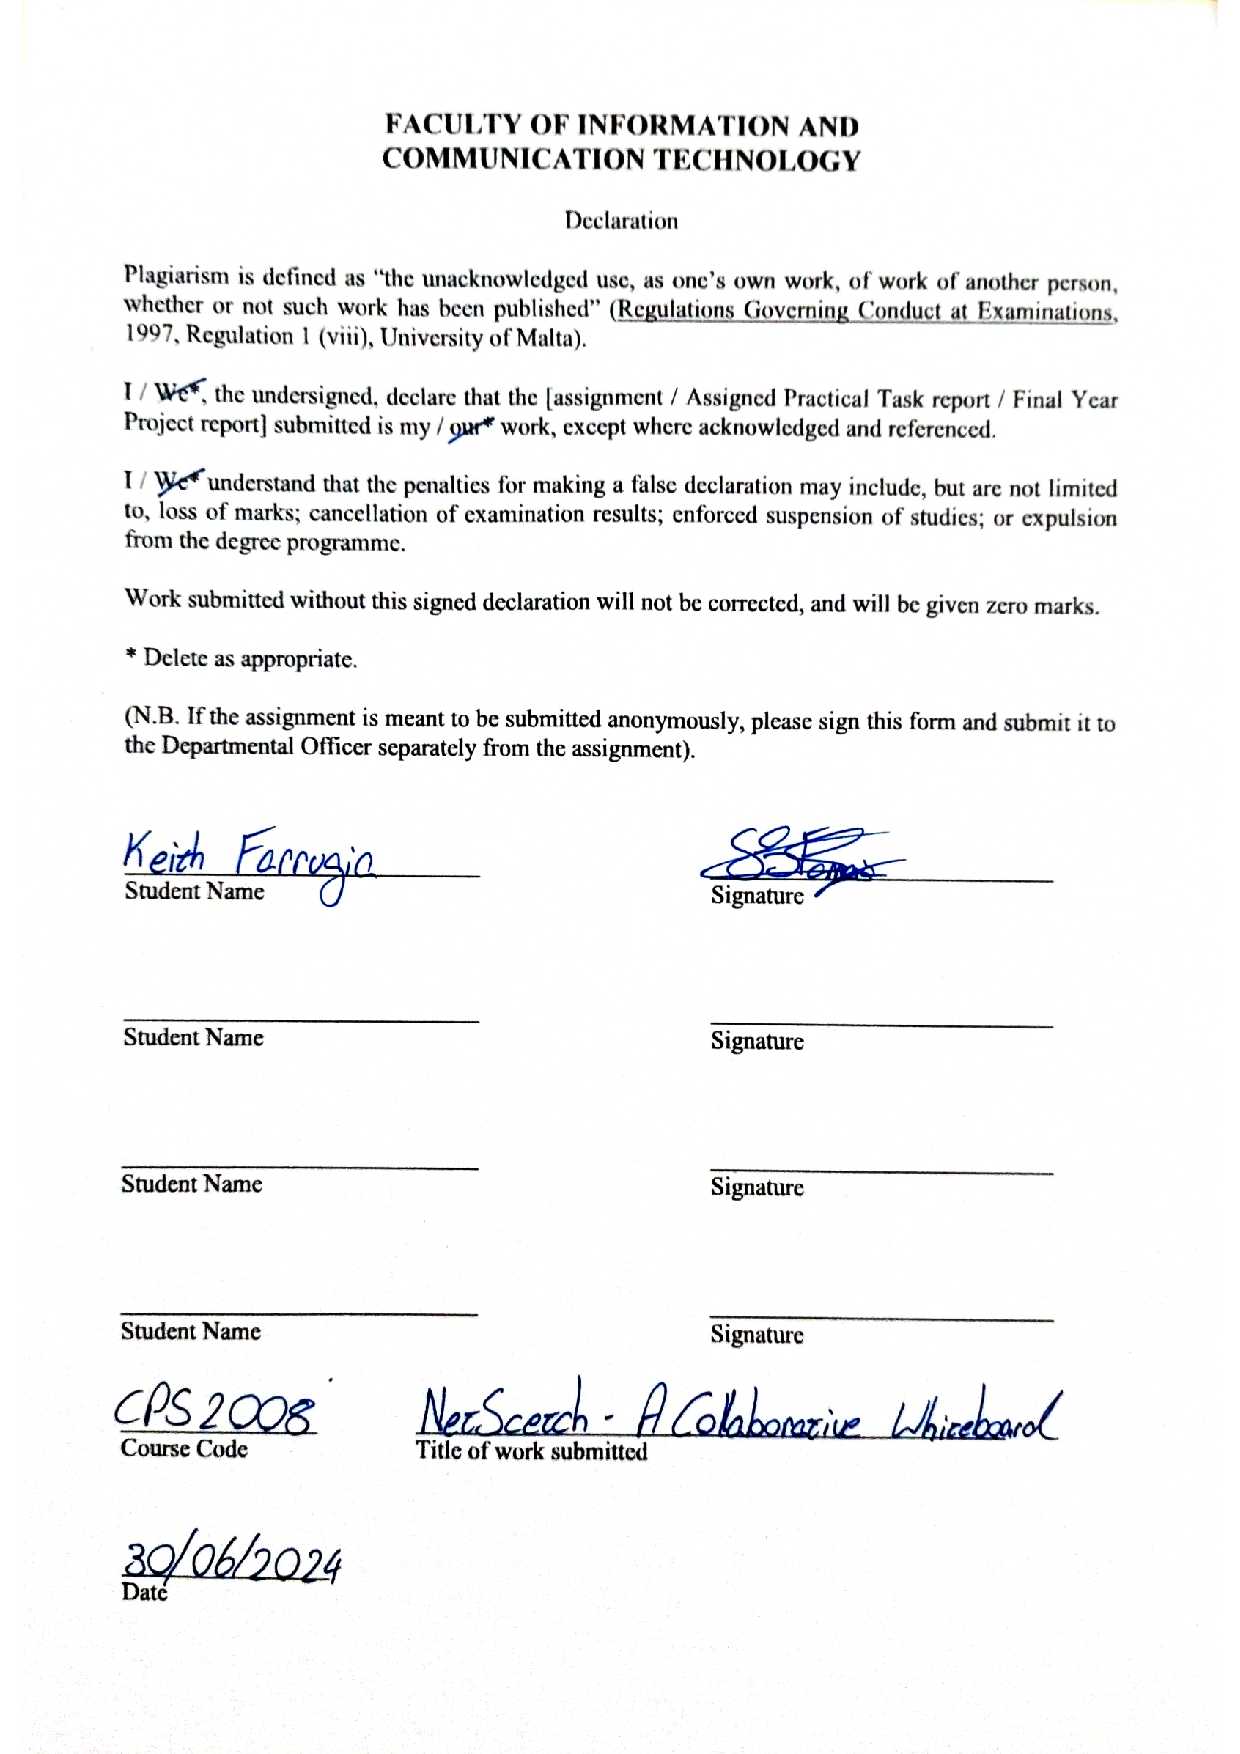
\includepdf[pages={1}]{Plagiarism Form - Keith Farrugia 11104L.pdf}

\chapter{Introduction}
\section{Links}

\textbf{Video link:} \url{https://drive.google.com/file/d/1V6SQK9D63EtJWdg4Ptz-nzjBbVSKRhWl/view?usp=sharing}

\section{Building}
The system requires quite a few libraries in order to compile properly. As well as some steps which need to be made before compilation must be done. Below are the steps to ensure that everything is in order.

\subsection{Libraries}
The table below shows the libraries needed and their commands.

\begin{table}[ht]
    \centering
    \renewcommand{\arraystretch}{1.5}
    \setlength{\tabcolsep}{12pt}
    \begin{tabular}{
        |> {\raggedright\arraybackslash}p{0.10\linewidth}
        |> {\raggedright\arraybackslash}p{0.10\linewidth}
        |> {\raggedright\arraybackslash}p{0.30\linewidth}
        |> {\raggedright\arraybackslash}p{0.30\linewidth}
    |}
        \hline
        \textbf{Library} &  \textbf{Reference} &\textbf{Command} & \textbf{Description} \\ \hline
        
            Build Essentials                                                &
            \cite{GCC}                                                      &
            \texttt{sudo apt install -y build-essential cmake}              &
            This downloads the latest Cmake and C++ compiler(GCC)           \\ \hline
            
            SDL2                                                            & 
            \cite{SDL}                                                      &
            \texttt{sudo apt install -y libsdl2-dev}                        &  
            This downloads the SDL library which is used for 
            drawing and launching the window                                \\ \hline
            
            SDL2\_ttf                                                       &
            \cite{SDL_TTF}                                                  &
            \texttt{sudo apt install -y libsdl2-ttf-dev}                    &
            This downloads the text rendering extension for SDL             \\ \hline
            
            SDL2\_gfx                                                       &
            \cite{SDL2_gfx}                                                 &
            \texttt{sudo apt install -y libsdl2-gfx-dev}                    &
            This downloads the extension which allows for the
            rendering of more complex geometric shapes                      \\ \hline
            
            Protobuf                                                        &
            \cite{Proto}                                                    &
            \texttt{sudo apt install -y protobuf-compiler libprotobuf-dev}  &  
            This is the serialization library which is used to create and
            send the packages as well as draw item lists                    \\ \hline
            
            OpenSSL                                                         &
            \cite{OpenSSL}                                                  &
            \texttt{sudo apt install -y libssl-dev}                         &  
            This is a cryptographic library used to generate the hash
            seen in the tests                                               \\ \hline
    \end{tabular}
    \caption{Libraries and their installation commands}
    \label{tab:libs}
\end{table}

\newpage
Alternatively, the code repository comes with a script "install\_libraries.sh", which will automatically install the needed libraries (feel free to change it to choose what libraries to install).That being said the script does not install Cmake or GCC. Follow the steps below in order to run the script:

\begin{enumerate}
    \item Open the terminal and 'cd' or set the directory to the folder where the script is located.
    \item \textbf{Run:} chmod +x install\_libraries.sh
    \item \textbf{Install:} ./install\_libraries.sh install
    \item \textbf{UnInstall:} ./install\_libraries.sh uninstall
\end{enumerate}

\section{Build Setup}
There are also other configurations needed before the repository can be built.


Firstly the font used in the text rendering needs to be located in the build file. This can be done by refreshing the Cmake list. This is usually done by saving the Cmake list (at least in Visual Studio). If this is done correctly then a "fonts" folder should appear in the build directory holding the SpaceMono-Regular.ttf file [Figure: \ref{font}].

\begin{figure}[!htp]
    \centering
    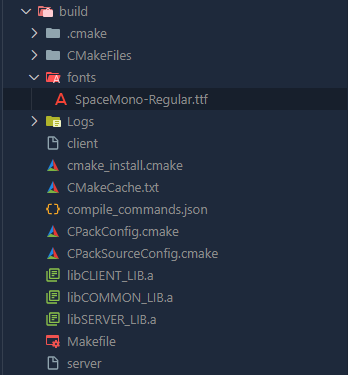
\includegraphics[width=4cm]{FontsFile.png}
    \caption{Font file in build}
    \label{font}
\end{figure}


Secondly, the protobuf files need to be generated. This can be done through the following steps:
\begin{enumerate}
    \item Open the terminal and 'cd' to the repository.
    \item Further set the current directory (using 'cd') to be the following "Common/Serialize".
    \item If you were to view the files, the "Serialize.proto" file should be visible.
    \item \textbf{Run:} \begin{verbatim}protoc --cpp_out=. Serialize.proto\end{verbatim}
    \item This should generate 2 new files: "Serialize.pb.cc" \& "Serialize.pb.h" [Figure: \ref{protobuf}],
\end{enumerate}

\begin{figure}[!htp]
    \centering
    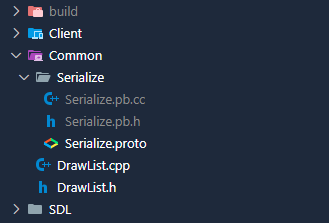
\includegraphics[width=5cm]{Protobuf.png}
    \caption{Protobuf generated files}
    \label{protobuf}
\end{figure}

Now the Repository can be compiled and no errors should occur.
%========================================================================================
%========================================================================================
\chapter{General Overview}
The following section gives a brief overview of general concepts, giving an overview of what is going on without going into the specific details. This should help in understanding the more in-depth explanations later on.

\section{Command processing}
The figure below [Figure: \ref{GCSC}] shows the general process of client-to-server-to-client communication. The server mostly acts as a relay for the commands and a record holder of the current draw list. This limits the stress on the server as most of the menial work is done by the users.
\begin{figure}[!htp]
    \centering
    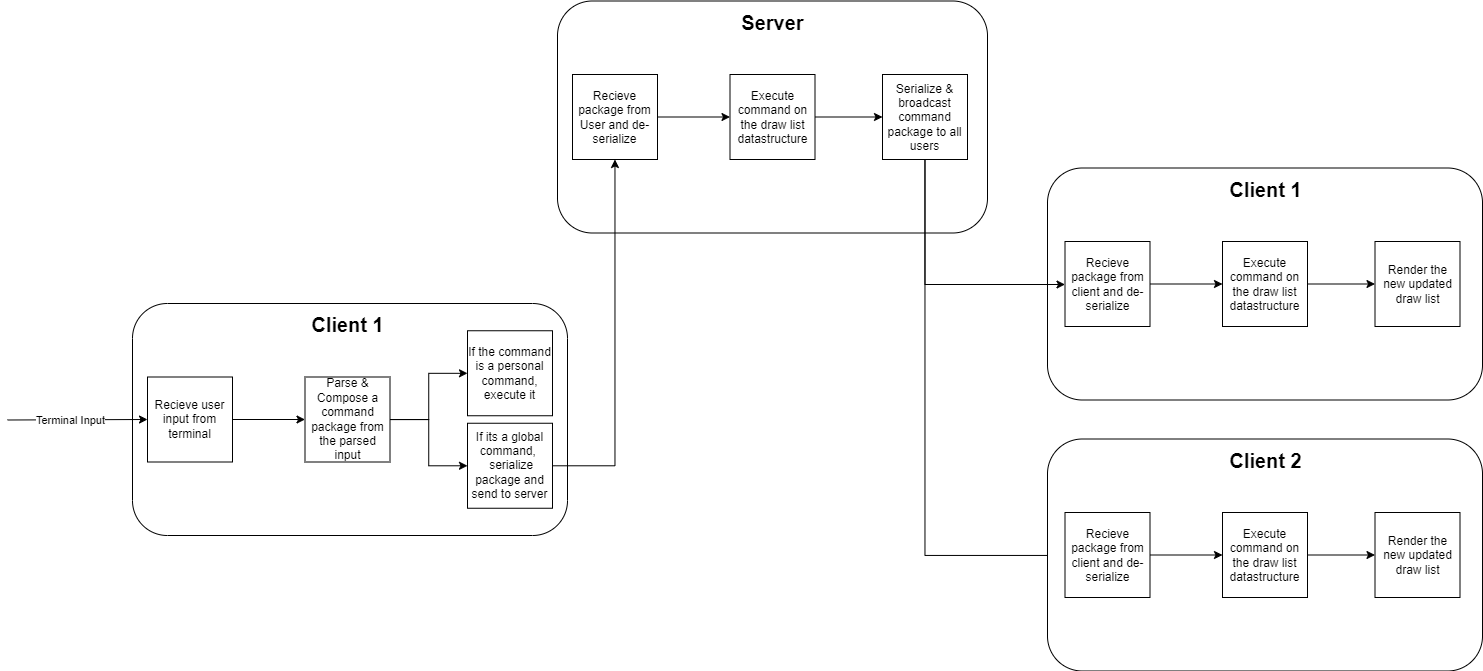
\includegraphics[width=15cm]{Server To Client General.drawio.png}
    \caption{General client to server to client overview}
    \label{GCSC}
\end{figure}

\section{Re-Connect \& New Client Events}
The re-connect or new-client event can be seen visually in the figure below [Figure \ref{RC}]. This is again only a surface-level explanation, concepts such as validation and the like are not discussed.
\begin{figure}[!htp]
    \centering
    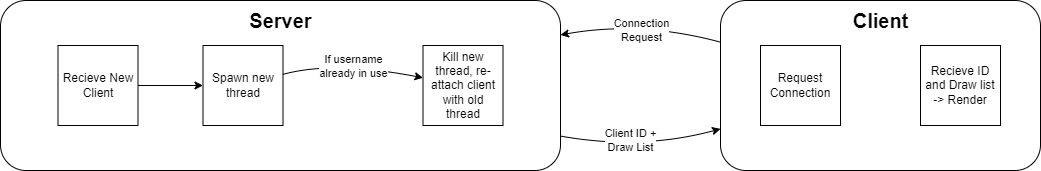
\includegraphics[width=15cm]{Re-Connect Event.drawio.png}
    \caption{Re-Connect Event}
    \label{RC}
\end{figure}

\chapter{DrawList}
The draw list data structure is common among all clients and server components. The main purpose for its creation is to allow quick execution of the commands related to the list of draw functions. Since the data structure functions are common throughout, it means that all commands should be executed in the same way by all parties.

The draw list data structure itself is made from a map which allows for quick access to the singular operation such as insertion and editing. This also allows for ordered traversal based on the draw ID. This means that even if the draw items are inputted in a random order, the traversal will always result in the same representation or render on the canvas. The points below list the Big O notation of the important functions.

\begin{itemize}
    \item \textbf{insert:} $O(log n)$
    \item \textbf{erase:} $O(log n)$
    \item \textbf{edit:} $O(log n)$
    \item \textbf{traverse:} $O(n)$
    \item \textbf{list:} $O(n)$
    \item \textbf{undo:} $O(n)$
    \item \textbf{serialize:} $O(n)$
    \item \textbf{load:} $O(n)$
    \item \textbf{generate\_hash:} $O(n)$
\end{itemize}

The draw list structure itself is also built around the protobuf generated components, This makes it easier to serialize and de-serialize the list from transition over the TCP connection. Additionally, the data structure ensures that no invalid commands are executed on the data structure. For example, if 2 clients were to attempt the deletion and editing of a draw item, no issues would arise. This is also further ensured by the fact that the data structure itself has inbuilt mutex locks which ensure that at most only 1 thread can manipulate the data.


\section{Command Description} \label{Commands}
\begin{itemize}
    \item \textbf{insert:} A new PB\_DrawData item is added to the map.
    \item \textbf{erase:} The PB\_DrawData item matching the same draw ID is removed from the map.
    \item \textbf{edit:} The PB\_DrawData item matching the same draw ID is replaced with the new PB\_DrawData item.
    \item \textbf{traverse:} Each PB\_DrawData item is traversed in order depending on the draw ID and each is passed to the function pointer passed as a parameter.
    \item \textbf{list:} Displays all PB\_DrawData items in order of draw ID and prints those who match the parameters.
    \item \textbf{undo:} Given a user ID it removes the latest PB\_DrawData item, meaning the highest draw ID, belonging to that user.
    \item \textbf{serialize:} Transfers the entire map to a protobuf list to be serialized.
    \item \textbf{load:} Loads a given protobuf list replacing all entries in the current map.
    \item \textbf{generate\_hash:} Generates a hash value depending on the serialized version of the PB\_DrawData items 
\end{itemize}

%========================================================================================
%========================================================================================
\chapter{Client}


\section{Structure}
The client itself is made up of 3 threads (including the main thread). At the start, only 2 threads (including the main thread) were used, where the main thread handled the terminal input and sent packages to the server. The second thread used to be for receiving commands from the server, executing and then rendering the updated whiteboard. 

Even though this did suffice for a basic simulation of a couple of clients, during the stress testing it seemed that the clients were unable to keep up with the amount of traffic, at least when a large number of clients were sending messages at the same time. Hence the second thread was split into a further 2 threads one that tries to empty the socket buffer as quickly as possible while the other executes and renders.

\section{Client Launch}
In order to launch the client 3 to 4 parameters must be set:
\begin{itemize}
    \item \textbf{--server <IP address>} : Specify the ip address for the server.
    \item \textbf{--port <port number>} : Specify the port number for that server.
    \item \textbf{--nickname <artist name>} : Specify the username for this client.
    \item \textbf{[--test]}: An optional test parameter that if passed no outputs from the client will be made except during termination where a hash value is generated from the draw list and displayed.
\end{itemize}

The client will then attempt to connect to the server sending the username and receiving the server-assigned ID. After which the 3 threads are launched or executed.



\section{Main Thread}
\subsection{Parsing}
Contrary to the requirements the command parsing from the raw input was done on the client side of the process. This made more sense since there wasn't a point for the commands to be parsed on the server for each client. This would only serve to place more stress on the server component. Instead, the clients parse the command and create a package in an easily readable format through proto buffers.

\subsection{Lexer \& DFSA}
The parsing is done by re-using a Lexer component from a different assignment (CPS2000). It works as a character reader and tokenizer implemented through the creation of a Dynamic State Finite Automata (DFSA). The DFSA itself can be seen in the Figure provided [Figure \ref{DFSA}].
\begin{figure}[!htp]
    \centering
    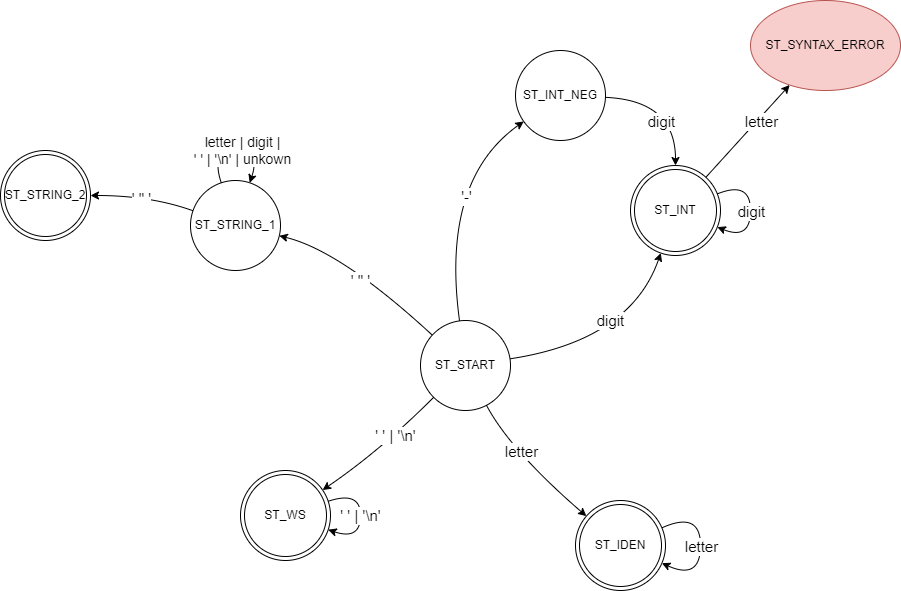
\includegraphics[width=15cm]{NetScetch DFSA.drawio.png}
    \caption{DFSA}
    \label{DFSA}
\end{figure}

In short, the Lexer works by traversing each given character, assigning a lexeme which is then used to deduce the next state in the DFSA. This is done until the Lexer reaches an undefined state at which point it rolls back to the last exceptible state and tokenises that substring. There is a special case for identifiers where each is further tokenised depending on the command such as with "draw", "select", "delete", etc.

\textbf{Note:} The Lexer does not accept floating point numbers since the addition of such numbers would not be visible when drawing due to the view ratio of the canvas.

\subsection{Command Creation}
The user input is, as mentioned before, tokenised through the Lexer and then parsed. The functions are located in the "Client/User\_Functionality/Parse\_Commands.cpp" file. Here depending on the first keyword, the relative handler for the expected command is called which validates and constructs the required package for the server, or required execution steps. The clients never execute user commands directly except if the commands do not affect the draw list. 6 commands are executed directly; exit, colour, select, list, and show. The following is a brief explanation of how each command is handled. It is important to note that the commands all result in the same package structure. This can be seen through the structure specified in the ".proto" file located at "Common/Serialize".

\begin{itemize}
    \item \textbf{Help:} Commands are listed together with the expected parameters and a small description.
    \item \textbf{Tool:} Sets a static variable to hold the selected tool.
    \item \textbf{Colour:} Sets a static PB\_Colour variable to the current colour.
    \item \textbf{Draw:} Depending on whether a draw\_id has been selected or not the function creates a package that is then sent to the server. This can either be an "insert" type package, or an "edit" type package, either way, both hold a PB\_DrawData object which is what is held in the drawlist. 
    \item \textbf{List:} Depending on the parameters a list of draw items are printed. This is done from the functions provided in the draw list data structure.
    \item \textbf{Select:} A static integer is set to hold the selected draw ID.
    \item \textbf{Delete:} A delete package is sent to the server with a draw ID.
    \item \textbf{Undo:} An undo package is sent to the server.
    \item \textbf{Show:} A static variable is set to represent what the user has selected to be shown in the window. Another variable "should\_render" is also set in order to refresh the Canvas.
    \item \textbf{Clear:} A clear package is sent to the server, including a draw ID.
    \item \textbf{Exit:} A kill flag is set and both threads are shut down.
\end{itemize}



\section{Server Thread}
As mentioned before during stress testing the clients seemed to fail when it came to keeping up with the amount of traffic sent by the server. In other words, the server was sending so many messages that clients would not be able to clear the socket's message buffer in time and so would lose command packages due to overflow.

However, this most probably was due to the fact that there were so many threads running during the stress test that the operating system was not assigning enough time to each. This is not really a huge problem since in reality it's impractical and not likely that a single computer would need to launch so many applications since each client would be launched from a different machine.

Still, an attempt to nullify this was made by creating a thread whose sole purpose is to try and empty the socket buffer as quickly as possible. No decoding or execution of the instructions is made, but simply transferring from the socket buffer to a queue in order to limit the overflow. This did significantly improve the results by around 70\%. Although it's still not a perfect system it should be enough to handle a large amount of clients when in a more realistic setting.


\section{Rendering Thread}
The purpose of the render thread is to work in tandem with the server thread and clear the message queue, by decoding and executing each command package stored. A secondary function is rendering the canvas in order to show the continuous real-time view of the current whiteboard.

\subsection{Command Execution}
In order to ensure synchronization the clients are unable to execute draw-related commands themselves unless they receive them from the server. This ensures that all clients receive a given command and so all clients are on the same wavelength. This approach is to try and prevent de-synchronization rather than detecting it and fixing it.

In terms of actual command execution, it is fairly simple since each command has its own drawlist equivalent function which is then called with the required information. To better understand what the commands do its best to refer to the section draw list command section, i.e. Section \ref{Commands}

\subsection{Rendering}
In order to generate and render the canvas, the project makes use of the external library known as SDL \cite{SDL} together with two other libraries which extend it; SDL\_TTF \cite{SDL_TTF} and SDL\_gfx \cite{SDL2_gfx}. The reason why these libraries were used is the following:

\begin{itemize}
    \item \textbf{SDL\_TTF:} Text rendering, so that the string inputted by the user can be translated into textures and rendered on the screen. As well as reading and using the chosen font from Google fonts \cite{SPACE_MONO}.
    \item \textbf{SDL\_gfx:} Used for shape generation, allowing for easy creation of rectangles, lines and circles.
\end{itemize}

In order to give the illusion of a continuous whiteboard, the mouse clicks and drag events are recorded to move the virtual viewpoint around. From here the positions for each item are adjusted in order to shift their location on the screen giving the impression that the user is moving about in a 2D space. In order to provide a reference point rulers are also being drawn on top of the rendered items. The rulers work by drawing lines/markers at set intervals with textboxes showing the relative locations. These are also shifted based on the user's viewpoint but once a marker reaches the end of the visible positions, it is removed and a new marker is placed in the opposite location.






%========================================================================================
%========================================================================================
\chapter{Server}
In order to make sure that the load of each client is split as evenly as possible, the server makes heavy use of threads. In fact, each client has its own client-handler thread dedicated to it by the server. There is still only a singular draw list, which only ever lets a single thread access it at any time, but the multiple threads aid in de-serializing and re-serializing packages as well as broadcasting them. Although similar to the list, the server only allows a single thread to broadcast at a given time.

\section{Server Launch}
In order to launch the server a port must be specified. If this port is not in use, the server creates a TCP connection and starts listening to client connections. The basic process of how the server works is that the main thread listens for new connections, with it creating a new client-handler thread for that connection. The server's main loop allows up to 100 users to be in the connection queue meaning that it allows up to 100 connections to be in the queue (not yet assigned a thread) before new connections are ignored.

A secondary purpose for the main loop is to take user input from the terminal, more specifically it also listens for the user to input the exit command initiating the server's termination. If the server is terminated, the client threads all get notified through a flag and each shutdown on its own. The main thread will wait until all threads have been shut down/killed before terminating itself. Upon the server's termination, clients receive an invalid message automatically which also terminates the client processes since there is no longer a server to connect to.

\section{Client Handler Thread}
The first the client handler thread does is receive the username sent by the client. It is assumed that the client can be identified through their username, meaning that two \textit{active} clients can have the same username. If the username is in use by an active client then an error message is sent to the client and the connection is terminated. If the username is used by an inactive client then it is assumed that this new connection is simply a reconnect attempt made by the client. In this case, the thread updates the client's status to active and updates the socket number and the thread terminates allowing the old thread to reconnect with the client. If this is a new connection then the thread continues on creating a new client entry into the client list.

Upon verifying the new client, the current draw list data structure is sent to bring the client up to speed with the current state of the server's canvas. The thread will then move on to polling the socket for client messages. If a message is received then the thread reads and decodes it. Else the thread will move to other tasks. Either way, the thread will also be on the lookout for any change in the kill flag to terminate when the server orders it.

\subsection{Successfull Message}
In the case that the received message is successfully read, the thread de-serializes and adds it to a buffer of messages, and moves on to trying to read the next message. In the case that the message is an insert command, a draw ID is assigned through the use of the global static draw ID counter. Messages are stored in a buffer to accommodate scenarios where a user sends multiple messages in quick succession. By temporarily holding these messages, the system can clear the socket's buffer, thus preventing overflow. This buffering mechanism allows the system to process the messages at a more manageable pace, particularly when the system is under heavy load, providing greater flexibility and stability overall.

\subsection{Unsuccessfull Message}
If there is an error that arises during the reading of the message, it is usually caused by the client disconnecting. In this case, the thread waits for the user to reconnect. This is done by checking the status of the client in the client list. If the client were to reconnect then another thread would set the client's activity to active. If the status has not changed, the thread sleeps for 1 second and checks again. This is done until the thread reaches around 1 minute of waiting time at which point the thread removes the client's data from the client list, allowing the username to be reused by a different client, and the thread terminates. If the client does re-connect, the server's draw list is packaged and sent to them to bring them up to speed.

\subsection{No Message Recieved}
In the case that the user doesn't receive a message by the time the poll's time limit is up, it will try to empty its buffer of messages. Here the main draw list is accessed and the command is executed. After the draw list is updated, the command package is re-serialized and broadcasted to all clients including the one which sent it, so that all can update their own lists. It is important to note that if a thread is not able to obtain the mutex lock within a time limit, then the thread goes back to see if the user has sent any messages. Repeating the cycle.

\subsection{User disconnect}
One important thing to mention is the case of what happens when a user disconnects. The actual procedure is listed above through code explanation, but in short basically, if a user disconnects they have 10 minutes in which they can try to re-connect. If they are not able to re-connect in that time then the client handler thread is killed, and a different client can reuse the username.

It is important to note that although the requirements say that the server should absorb commands from disconnected clients, this was not implemented directly. This is because something similar is already in effect due to how the system is implemented. Since the ID for that client will never be used again it is technically the same as having the server absorbing those commands. Additionally, since you cannot query any function by the server (since the only options are ALL or MINE), there is no point in going through and re-assigning IDs to those commands which would symbolize ownership to the server.

\subsection{Inactivity}
Another feature that the server has is that users who have been inactive for 10 minutes are sent an error message which will automatically kick them from the server. However, there is still a minute for them to reconnect. This is done by taking the last time the user was active and periodically checking if 10 minutes have passed since then.


\chapter{Performance and Testing}
In the following section, I will be discussing the tests, overall performance, and some statistics.

\section{Basic Statistics}
The following are some statistics which was gathered during testing about the protobuf-generated objects used. For these statistics to be generated sample objects were created and their sizes were then calculated.


\subsubsection{Explanation Code Snippit}
The code snippet below shows how such statistics were gathered in order to understand what the statistics mean

\begin{minted}[frame=lines,framesep=2mm,baselinestretch=1.2,bgcolor=LightGray,
fontsize=\footnotesize,linenos,breaklines=true]{c++}
    PB_DrawCircle circle;
    circle.set_x(10);       circle.set_y(20);
    circle.set_radius(5);   circle.set_filled(true);
    
    PB_Colour* color1 = circle.mutable_colour();
    color1->set_r(255);     color1->set_g(0);
    color1->set_b(0);       color1->set_a(255);

    PB_DrawData draw_data1;
    draw_data1.set_user_id(1);
    draw_data1.set_draw_id(1);
    *draw_data1.mutable_circle() = circle;

    PB_Package package1;
    package1.set_message_type(PB_INSERT);
    *package1.mutable_draw_data() = draw_data1;
    
    std::court 
        << "Size of draw_data1 (circle): " 
        << draw_data1.ByteSizeLong() 
        << " bytes\n";

    std::court 
        << "Size of package with draw_data1 (circle): " 
        << package1.ByteSizeLong() 
        << " bytes\n";
\end{minted}




\subsubsection{Objects Tested}

\begin{table}[h!]
\centering
\begin{tabular}{|p{0.3\linewidth}|p{0.6\linewidth}|}
\hline
\multicolumn{1}{|c|}{\textbf{Object}} & \multicolumn{1}{c|}{\textbf{Details}} \\ \hline
\textbf{Circle} &
\begin{tabular}{l}
    x = 10 \\
    y = 20 \\
    radius = 5 \\
    filled = true \\
    colour = (255, 0, 0, 255)
\end{tabular} \\ \hline
\textbf{Line} &
\begin{tabular}{l}
    x = 10 \\
    y = 20 \\
    x\_to = 30 \\
    y\_to = 40 \\
    colour = (0, 255, 0, 255)
\end{tabular} \\ \hline
\textbf{Rectangle} &
\begin{tabular}{l}
    x = 30 \\
    y = 30 \\
    width = 50 \\
    height = 50 \\
    filled = true \\
    colour = (0, 0, 255, 255)
\end{tabular} \\ \hline
\textbf{Text} &
\begin{tabular}{l}
    x = 50 \\
    y = 60 \\
    text = "Hello, World!" \\
    colour = (255, 255, 0, 255)
\end{tabular} \\ \hline
\end{tabular}
\end{table}

\subsubsection{Draw Data Statistics}
The following are the statistics of the PB\_DrawData objects holding the above-mentioned data.



\begin{itemize}
    \item Size of draw\_data1 (circle): 22 bytes
    \item Size of draw\_data2 (line): 22 bytes
    \item Size of draw\_data3 (rectangle): 24 bytes
    \item Size of draw\_data4 (text): 34 bytes
\end{itemize}

\subsubsection{PackageStatistics}
The following are the statistics of PB\_Packages holding the above-mentioned draw data items as if they were insert command packages 


\begin{itemize}
    \item Size of package with draw\_data1 (circle): 26 bytes
    \item Size of package with draw\_data2 (line): 26 bytes
    \item Size of package with draw\_data3 (rectangle): 28 bytes
    \item Size of package with draw\_data4 (text): 38 bytes
\end{itemize}

\newpage
\section{Tests}

In terms of tests there are 3 tests:
\begin{enumerate}
    \item \textbf{Visual:} The visual test shows how a small subset of clients each with their whiteboard windows open. The point of these tests is to show visually that all the whiteboards reflect the same outcome.
    
    \item \textbf{Non-Visual:} These tests are more oriented to stress test the client-server connections. It is for this reason that the windows aren't launched, else the amount of windows needing to be rendered would take the bulk of the performance of the machine, and hence the test would reflect more on the efficiency of the SDL library rather than the implementation. As an additional note, the test doesn't reflect real-world scenarios as the chance of 100 clients needing to be run on a single machine is very low.

    In terms of how the result is determined this is done through hash values where clients given a test parameter will print out a hash value upon termination. By comparing these hash values it can be determined whether or not all clients have terminated with the same drawlist.

    The figure below shows the result of a successful stress test using the "Non\ Visual\ Parrallel\ Test\ Runner" [Figure: \ref{StressTest}]
    
    \item \textbf{Mixed Command:} This is a singular test and doesn't have a non-parallel alternative. This test server tests how different commands executed at the same time affect the clients and server. There are 3 clients that are launched; 2 test clients which will send the commands and a singular normal client which will act to show what is going on. 
    
    The primary goal of this test is to observe the behaviour of the server and clients when edit and delete commands are executed concurrently by two different clients. This helps us understand the impact of simultaneous command execution on the system's stability and performance.

    The result is determined the same way as the non-visual test where the hash values of the 2 clients are compared.
\end{enumerate}

\begin{figure}[!htp]
    \centering
    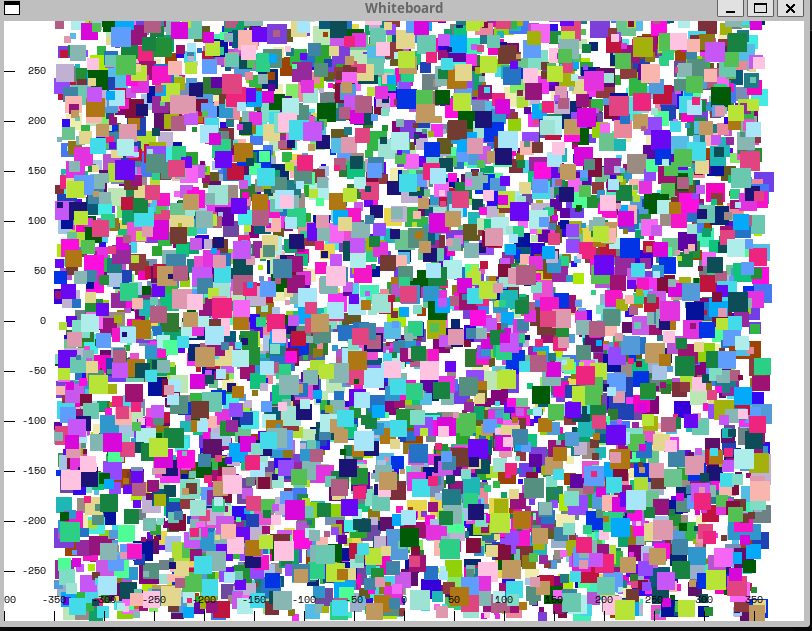
\includegraphics[width=10cm]{100 clients.PNG}
    \caption{100 Clients}
    \label{StressTest}
\end{figure}


It is important to note that each test has its parallel and non-parallel variants (except for the Mixed command test). The difference between the two is that the parallel tests use threads to pass the commands to the client's terminals meaning that all clients are being given commands at around the same rate leading to more stress being placed on the system.

The only test that is not always stable in its result is the non-visual-parallel-test, this most likely as mentioned before is more of an issue that the machine is not able to handle the amount of threads being launched (at least on the machine the implementation was made in).

In the video provided, you can view both tests and their results. Due to the time limit on the video, only the parallel tests were run since these were better at stress testing the system. The mixed commands test was also not run since it didn't fit in the time limit.


\textbf{[Important Note]:} When running the tests it is important to let the tests close the clients and server, else it is highly likely that the server may not get closed properly and will still be active after the python file is forcefully terminated.

\chapter{Possible Improvemets}
There are a lot of improvements that could have been made to the system but only the most important ones will be mentioned below.

\begin{itemize}
    \item The first improvement that could have been made is to reduce the amount of mutex locks used in the implementation. A lot of the mutex locks used were usually made redundant later on during the implementation. However, due to time constraints, there was not enough time to further debug the system and see what mutex locks could be removed.

    \item One major improvement that could be done is to implement some sort of synchronization checker into the system. As mentioned before the "Non\_Visual\_Parrallel\_Test\_Runner" is inconsistent when it comes to the results. Although it is again not an accurate real-world example, it is hard to not admit that the system does have a limitation due to the fact that if a de-synchronization does happen there is no current way to fix it.

    \item The undo is also something that could be further improved upon. A possible solution would be to add another parameter which would order items by last modified similar to the draw ID but which is also updated during editing.

    \item Another improvement would be the tests. Although the stress tests performed well for their purpose, better tests could have been made to show other functionalities. Unit tests could also have been implemented.
\end{itemize}


\bibliographystyle{IEEEtran}
\bibliography{bibliography}
\end{document}
